\chapter{Scaleability and Performance}

One of the most important motivating factor for writing a \CPP{} implementation
of the local search runtime was performance. The assumption was that the \CPP{}
implementation, even though it might have many restrictions, would be
considerably faster than the original Java one. Several performance benchmarks
were done throughout the development to verify or deny the previous statement.

\section{Model}

The model used during the performance benchmarks was an instance of the
previosuly introduced school metamodel (figure \figref{School_Metamodel}).
Table \tabref{model_size} shows the model scales used during performance
benchmarking.

\begin{table}[ht]
	\footnotesize
	\centering
	\caption{Model size}\label{tab:model_size}
	\begin{tabular}{ | l | c | c | c | c | c | c |}
	\hline
	Scale	& Schools	& Years & Courses	& Classes	& Students	& Teachers	\\ \hline
	1 		&  1		& 5		& 20		& 4			& 2000		& 10		\\
	2 		&  2		& 10	& 40		& 8			& 4000		& 20		\\
	4		&  4		& 20	& 80		& 16		& 8000		& 40		\\
	8		&  6		& 40	& 160		& 32		& 16000		& 80		\\
	16 		&  16		& 80	& 320		& 64 		& 32000		& 160		\\
	32		&  32		& 160	& 640		& 128 		& 64000		& 320		\\
	64 		&  64		& 320	& 1280		& 256 		& 128000	& 640		\\
	128 	&  128		& 640	& 2560		& 512		& 256000	& 1280		\\
	256 	&  256		& 1280	& 5120		& 1024		& 512000	& 2560		\\
	512		&  512		& 2560	& 10240		& 2048		& 1024000	& 5120		\\
	1024	&  1024		& 5120	& 20480		& 4096		& 2048000	& 10240		\\
	\hline
	\end{tabular}
	\label{tab:TabularExample}
\end{table}

The model size is defined with scale, which is essentially a simple multiplier
of the number of instances of each class defined in the metamodel. Larger
scales of a model simply created new instances of schools with similar
internal structure, but without any relationships not between the schools. The
instance model of a specified scale was generated using a deterministic
algorithm which was implemented in the same way in both Java and \CPP{},
allowing the comparison of the two framework implementation.

\section{Performance measurements}

The first measurements focus on the time it takes to initialize and execute a
query on a model, retrieving every match. The first pattern is the really simple
\emph{students} pattern \listref{meas_students}, which retrieves matches every
student in the model. The main difficulty for this pattern is that the result
set is very large (more than 2 million elements for the largest scale), this
means the main bottleneck is the creation of the result set itself.

\begin{lstlisting}[frame=single,float=!ht,language=IQPL,
label=listing:meas_students, caption=The students pattern]
pattern students(student) {
	Student(student);
}
\end{lstlisting}

Figure \figref{meas_students} shows the exution times measured for each platform
with different implementations and on three model sizes: 256, 512 and 1024. Java
LS refers to the local search implementation, while Java RETE refers to a
different, more mature pattern matcing implementation using the RETE algorithm
which provides incremental pattern matching capabilities.

\begin{figure}[!ht]
\centering
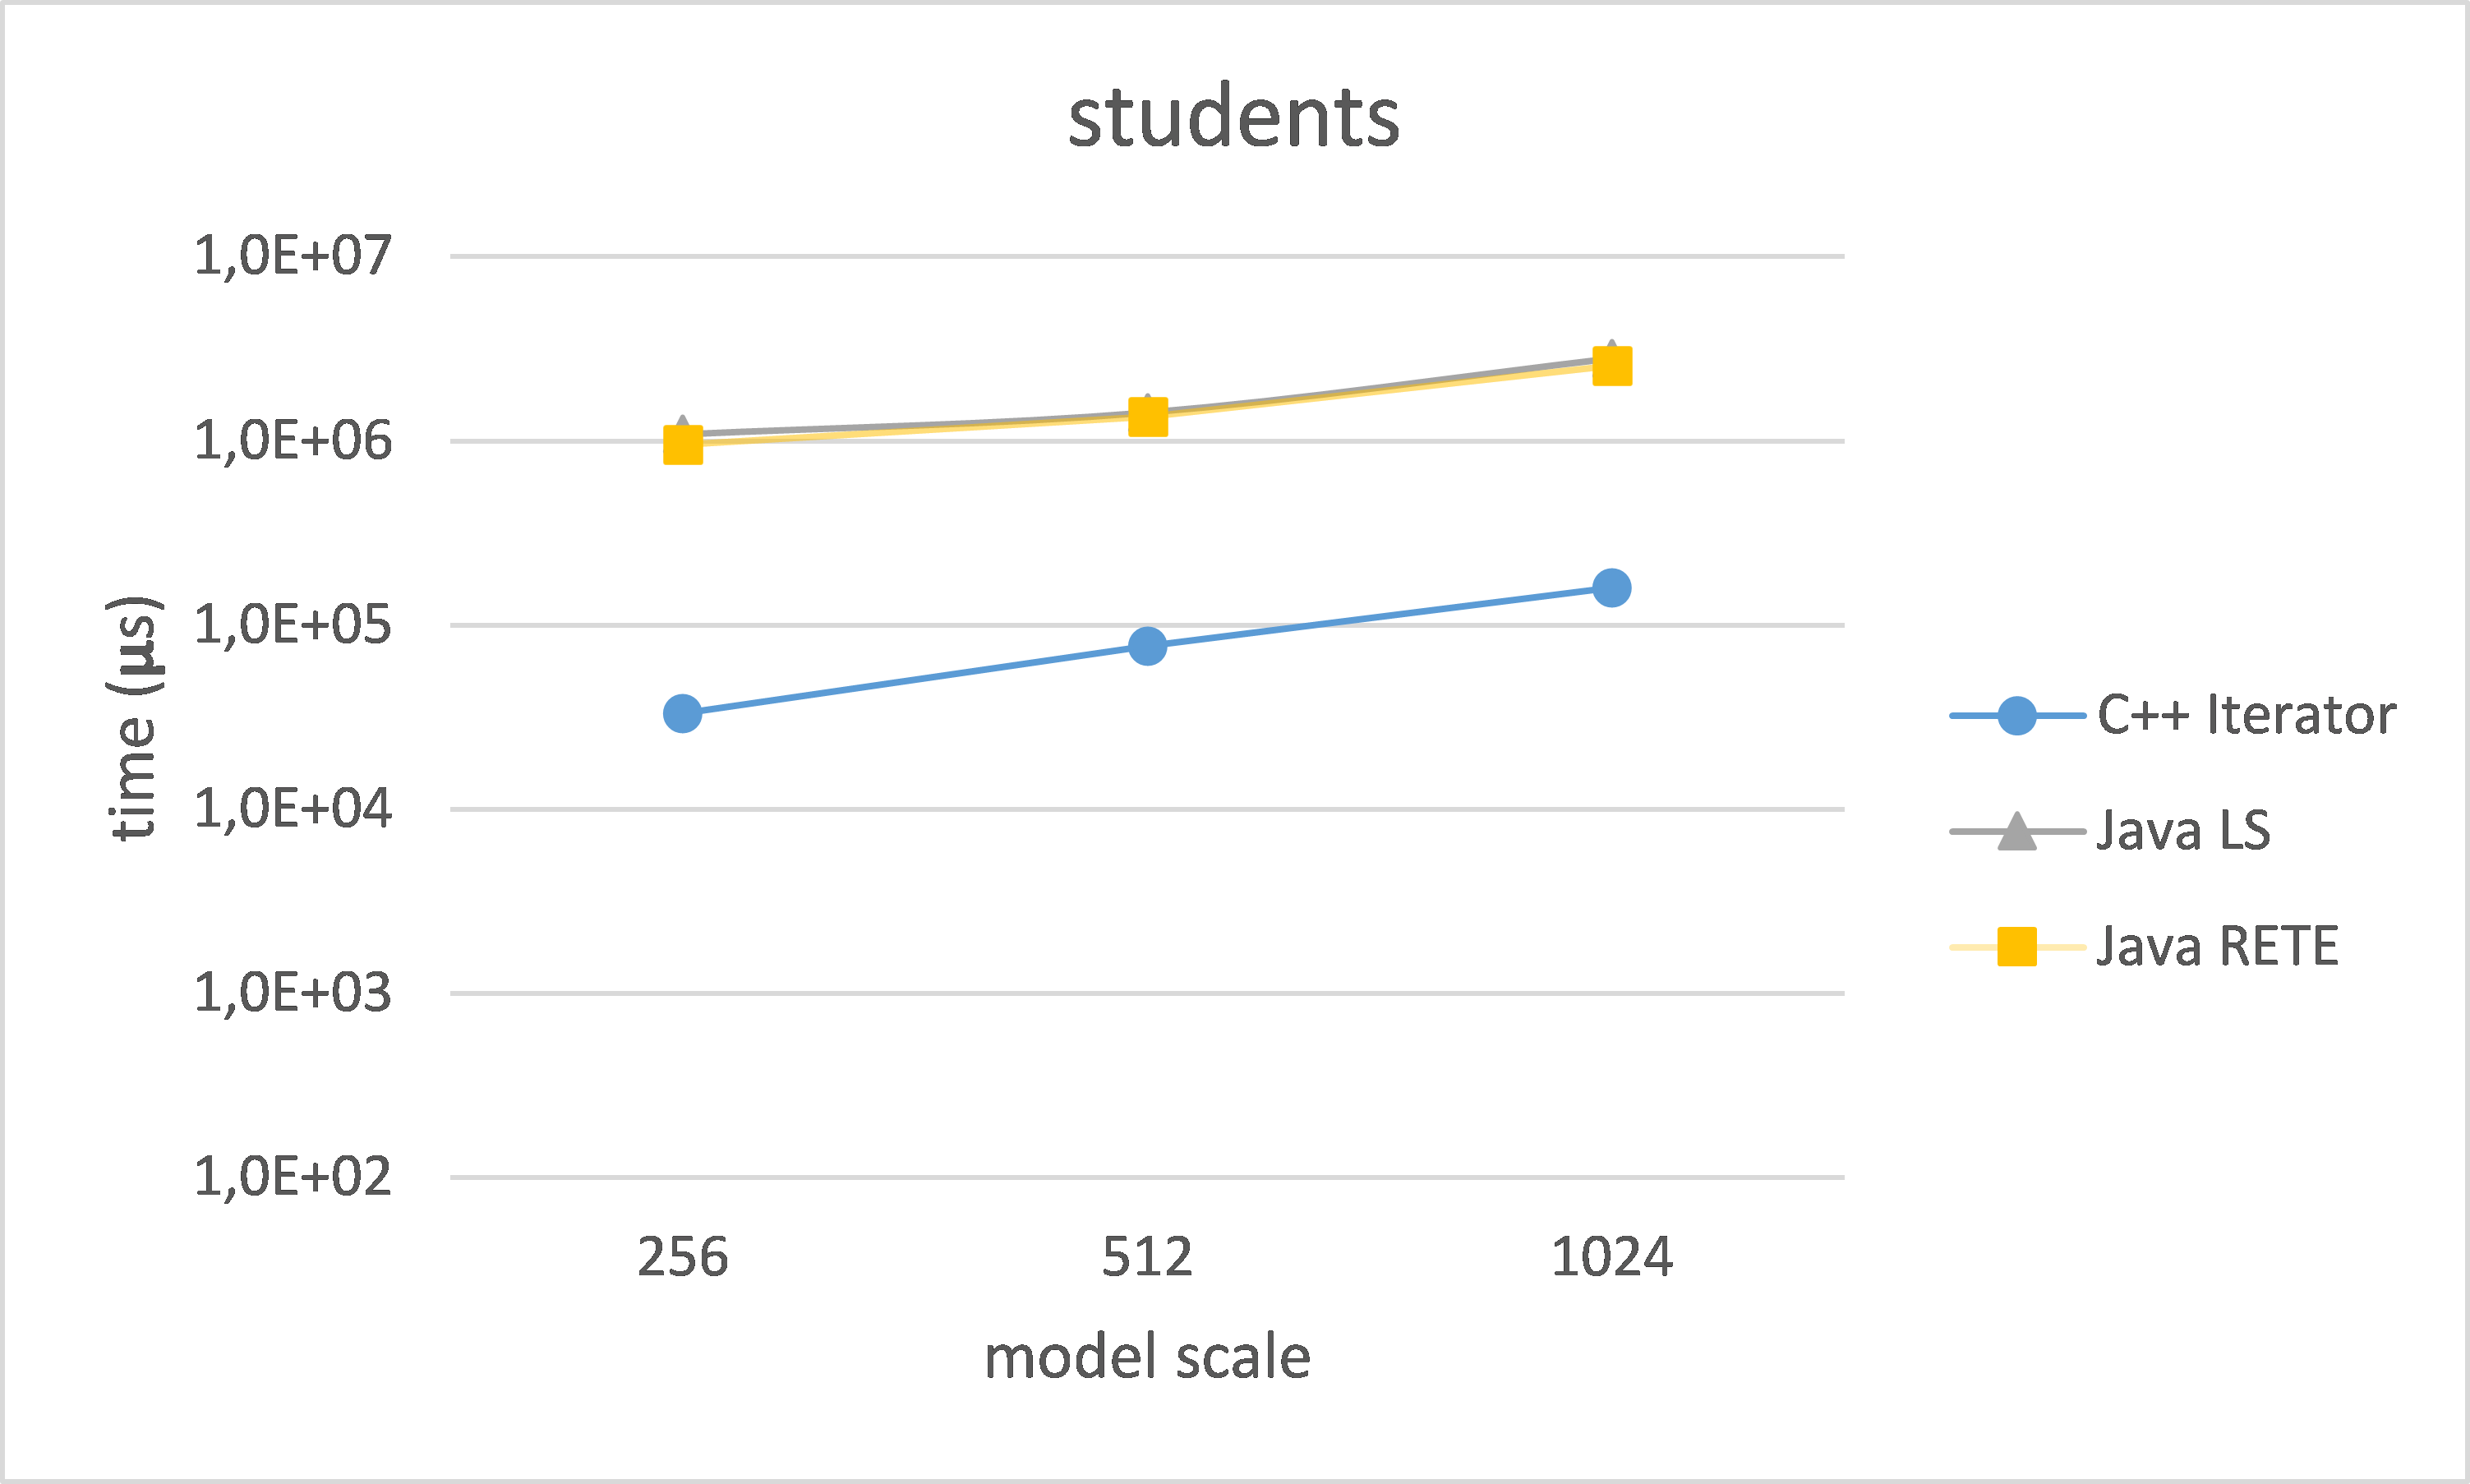
\includegraphics[width=120mm, keepaspectratio]{figures/meas_students.png}
\caption{Performance of the \emph{students} query}
\label{fig:meas_students}
\end{figure}

The measured times show the \CPP{} implementations performing considerably
better, then the Java ones. In the case of such a simple pattern this was
expected, as the \CPP{} implementation does a lot less preprocessing and most of
the query time consists of the assembly of the result set. The difference
between the iterator and runtime versions is very small, about 5-10\%. The
suprising part is the fact the Java implementation of the local search algorithm
does worse than the RETE based algorithm, which does a lot of advanced
preprocessing and caching. This could be the result of the immature codebase for
the local search based implementation, as it is still in development.

The next examined pattern is the \emph{classesOfTeacher} pattern
(\listref{meas_classesOfTeacher}). This pattern is slightly more complex than
the previous one, however the result set is really small. The main takeaway from
this benchmark is how fast an implementation can respond to a very simple query
with only a few tousand matches.

\begin{lstlisting}[frame=single,float=!ht,language=IQPL,
label=listing:meas_classesOfTeacher, caption=The classesOfTeacher pattern]
pattern coursesOfTeacher(course, teacher) {
	Teacher.courses(teacher, course);
}

pattern classesOfTeacher(teacher, schoolClass) {
	find coursesOfTeacher(course, teacher);
	Course.schoolClass(course, schoolClass);
}
\end{lstlisting}

The following chart (\figref{meas_classesOfTeacher}) shows the results of this
benchmark. In this case the \CPP{} implementations are still very close to each
other, but the difference between Java and \CPP{} implementations is absolutely
massive. The most probable reason is the preprocessing the Java implementations
do on the model, which results in the terrible return time. 

\begin{figure}[!ht]
\centering
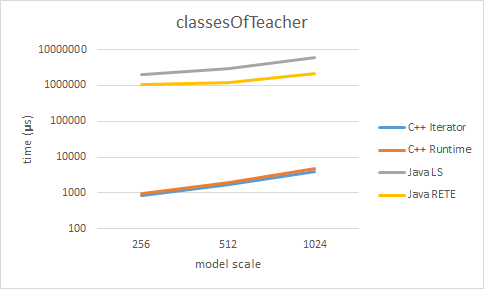
\includegraphics[width=120mm,
keepaspectratio]{figures/meas_classesOfTeacher.png}
\caption{Performance of the \emph{classesOfTeacher} query}
\label{fig:meas_classesOfTeacher}
\end{figure}

The Java local search implementation lags behind even more than the last time,
again, likely because of the not yet optimized code.

The next pattern is the \emph{studentsOfSchool}
(\listref{meas_studentOfSchool}), which is a moderately complex pattern. The
complexity comes from the fact that it is not possible to navigate through the
associations as described in the pattern because of the direction the
associations can be navigated in, thus the search plan has to overcome this via
starting from the center of the navigation chain and going in both directions
from there.

\begin{lstlisting}[frame=single,float=!ht,language=IQPL,
label=listing:meas_studentOfSchool, caption=The studentOfSchool pattern]
pattern studentsOfSchool(student, school) {
	Student.schoolClass.courses.school(student, school);
}
\end{lstlisting}

The more advanced pattern means the gap between the \CPP{} and Java
implementations became slightly smaller as seen on figure
\figref{meas_studentOfSchool}. As seen before, the Java local search
implementation lags behind the RETE implementation, while the \CPP{} iterator
and runtime based solution are roughly 5-10\% apart.

\begin{figure}[!ht]
\centering
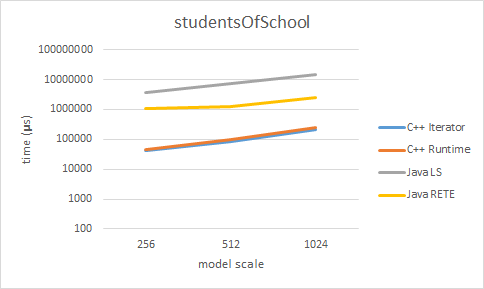
\includegraphics[width=120mm,
keepaspectratio]{figures/meas_studentOfSchool.png}
\caption{Performance of the \emph{studentOfSchool} query}
\label{fig:meas_studentOfSchool}
\end{figure}

The next pattern in line is the \emph{mutualFriendsInSchool}. This pattern is
the most complex of all the benchmarked patterns. The pattern searches for
two students in a single school whose friends with relationship is mutual. This
pattern is an absolute worst case scenario, as it calls an already complex
pattern twice resulting in a huge join at as the first steps of the search plan.

\begin{lstlisting}[frame=single,float=!ht,language=IQPL,
label=listing:meas_mutualFriendsInSchool, caption=The mutualFriendsInSchool pattern]
pattern mutualFriendsInOneSchool(studentA, studentB) {
	find studentsOfSchool(studentA, school);
	find studentsOfSchool(studentB, school);
	Student.friendsWith(studentA, studentB);
	Student.friendsWith(studentB, studentA);
}
\end{lstlisting}

In the case of this pattern the run times were a lot slower as expected,
which is why the times are written in milliseconds instead of microseconds
while the model scales are much smaller. The results, as seen on figure
\figref{meas_mutualFriendsInSchool}, do not continue the trend of the \CPP{}
version being faster than the Java implementation. In this case, both \CPP{}
implementations are slower then the Java RETE solution, while being slightly
faster than the Java local search version. The most likely reasons is a sub
optimal serch plan, which more than likely significantly hurt the performance
of all local search based solutions.

\begin{figure}[!ht]
\centering
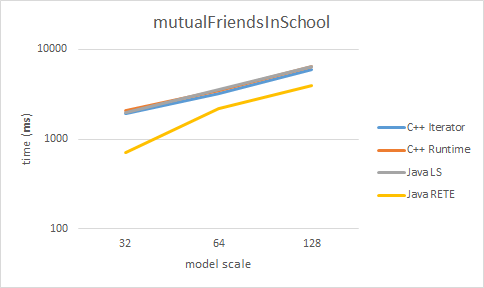
\includegraphics[width=120mm,
keepaspectratio]{figures/meas_mutualFriendsInSchool.png}
\caption{Performance of the \emph{mutualFriendsInSchool} query}
\label{fig:meas_mutualFriendsInSchool}
\end{figure}

The last figure (\figref{meas_second_run}) shows the times measured when running
the queries a second time. The pattern used in this benchmark is the
\emph{classesOfTeacher} (\listref{meas_classesOfTeacher}). In this case, the
\CPP{} implementations performed identical to the first run. The Java local
search based version shows slight massive improvements in its speed. The reason
for the speedup is that no perprocessing is necessary this time. The most
significant upgrade in speed is in teh case of the Java RETE algorithm based
solution, as the times dropped to constant 1 ms independent from the model size.
This is because of the caching and incremental updating this algorithm is
capable of.

\begin{figure}[!ht]
\centering
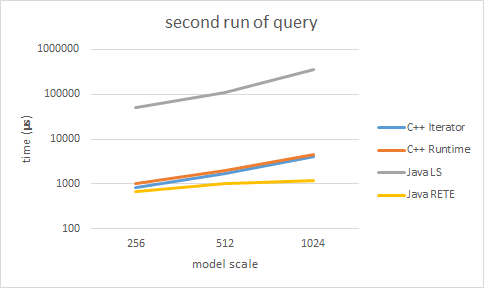
\includegraphics[width=120mm,
keepaspectratio]{figures/meas_second_run.png}
\caption{Performance of the second run of a query}
\label{fig:meas_second_run}
\end{figure}